\section{Experiment 3}\label{sec:experiment-3}
This experiment explores the differences in the kernels implemented in cross-validation regarding \gls{kpca}. Experiment 1, see \autoref{sec:experiment-1}, used the sigmoid kernel, and this experiment's goal is to assess whether the choice of the kernel could significantly impact the model's performance.

The configuration for the sigmoid kernel also used a different gamma value compared to the configuration for the \gls{rbf} kernel, which opens up researching the effect of the kernel and gamma for the model's accuracy. The experiment will focus on the confusion matrices and scores obtained from the different kernels.


\subsection{Rules and overview of the experiment}
The dimensionality reduction methods used in this experiment will be \gls{pca} and \gls{kpca}. The classification method will be \gls{svm}. The kernels used for \gls{kpca} will be \gls{rbf} and sigmoid.

The best configurations for each method used in this experiment is shown in \autoref{tab:best-configuration-expr-3}. The input of the data samples will be 15000 for both of the methods. The number of components used for all methods will be 49 components. The evaluation will be based on the confusion matrices and the results from the CSV file for cross-validation for \gls{kpca}. 


\begin{table}
    \centering
    \begin{tabular}{lrlll}
        \toprule
        method & components & C & parameter & parameter\\
        \midrule
        PCA-15 & 49 & C = 0.01 &  \\
        KPCA-15 & 49 & C = 1.0 & Gamma = 0.01 & Sigmoid \\
        KPCA-15 & 49 & C = 1.0 & Gamma = 0.001 & RBF \\
        % KPCA-15 & 49 & C = 1.0 & Gamma = 0.001 & Sigmoid \\
        % KPCA-15 & 49 & C = 1.0 & Gamma = 0.01 & RBF \\
        \bottomrule
    \end{tabular}
    \caption{Best configuration for each method used for experiment-3, method-15 means the method with 15 thousand samples.}
    \label{tab:best-configuration-expr-3}
\end{table}

This experiment is run on pc-2. See \autoref{tab:pc-specs} for the specific specs for the computer used in the experiment.

\subsection{Results}\label{subsec:experiment-3-results}
Below is shown the results for the methods. The results are in the form of confusion matrices. Accuracy percentages from the confusion matrices will compare the methods. The results for the two tests run on different $\gamma$ values are not presented as a confusion matrix, as the accuracy will only be compared, therefore the results are only shown in the CSV file and the discussion, see \autoref{subsubsec:gamma-influence}.

\subsubsection{PCA}
\begin{figure}[htb!]
    \centering
    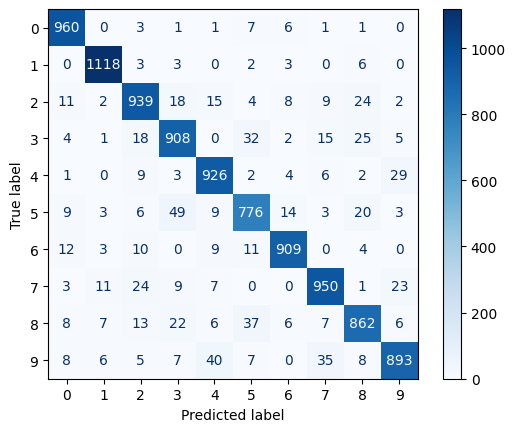
\includegraphics[width=0.8\textwidth]{figures/experiment-3/confusion_matrix_pca_svm.png}
    \caption{Confusion matrix for PCA}
    \label{fig:confusion-matrix-pca-svm}
\end{figure}


Figure~\ref{fig:confusion-matrix-pca-svm} shows the results for \gls{pca}. It has an accuracy of 92.37\%. It shows \gls{pca} is best at recognizing zeros and ones in pictures, as the model had guessed lees on the other numbers when the picture was zero or one. The model has trouble recognizing nines from fours and sevens, threes from fives, and fives from threes and eights.

\subsubsection{KPCA}

\begin{figure}
    \centering
    \subfloat[\centering Confusion matrix for \gls{kpca} Sigmoid]{\label{fig:confusion-matrix-kernel-pca-svm-sigmoid}{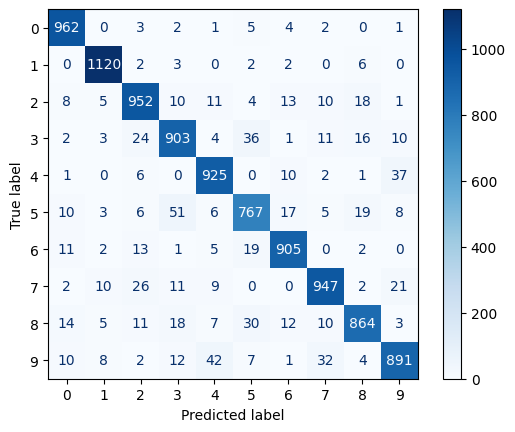
\includegraphics[width=0.45\textwidth]{figures/experiment-3/confusion_matrix_kernel_pca_svm_sigmoid.png} }}
    \qquad
    \subfloat[\centering Confusion matrix for \gls{kpca} RBF]{\label{fig:confusion-matrix-kernel-pca-svm-rbf}{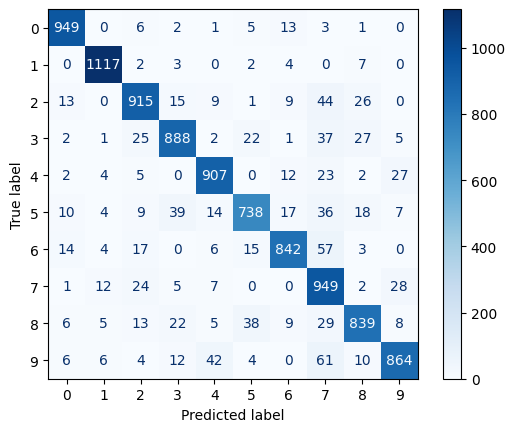
\includegraphics[width=0.45\textwidth]{figures/experiment-3/kernel_pca_rbf_kernel_49.png} }}%
    \caption{both \gls{kpca} kernels confusion matrices}
    \label{fig:kpca-kernels}
\end{figure}

Figure~\ref{fig:confusion-matrix-kernel-pca-svm-sigmoid} shows the results for \gls{kpca} with the sigmoid kernel. It has an accuracy of 91.50\%. It shows \gls{kpca-s} is best at recognizing zeros and ones in pictures, as the model had guessed lees on the other numbers when the picture was zero or one. The model has trouble recognizing nines from fours and sevens and tells threes, fives, and eights from each other.

Figure~\ref{fig:confusion-matrix-kernel-pca-svm-rbf} shows the results for \gls{kpca} with the RBF kernel. It has an accuracy of 89.5\%. It shows \gls{kpca-r} is best at recognizing zeros and ones in pictures, as the model had guessed lees on the other numbers when the picture was zero or one. The model has trouble recognizing nines from fours and sevens and tells fives, threes, and sevens from each other.

\subsection{Discussion of experiment 3}\label{subsec:discussion-experiment-3}
The results are compared two times, the best configurations on two kernels, where the main comparisons are in error percentage for each class, and last looking at the $\gamma$ hyperparameters influence on the results.

\subsubsection{Comparison of the best configurations}
From the results presented in Subsection\ref{subsec:discussion-experiment-3}, all the methods mostly confuse nines with fours and sevens. They also confuse threes with fives and sevens or eights. It can be further noted that \gls{kpca-r} is the worst at confusing various numbers with the number seven.

\begin{table}[htb!]
    \centering
    \begin{tabular}{lrrrr}
        \toprule
          & pca    & kpca-s & kpca-r \\
        \midrule
        0 & 2.959  & 1.836  & 3.163  \\
        1 & 1.585  & 1.321  & 1.585  \\
        2 & 8.817  & 7.751  & 11.337 \\
        3 & 10.594 & 10.594 & 12.079 \\
        4 & 5.702  & 5.804  & 7.637  \\
        5 & 12.556 & 14.013 & 17.264 \\
        6 & 6.054  & 5.532  & 12.108 \\
        7 & 7.101  & 7.879  & 7.684  \\
        8 & 13.552 & 11.293 & 13.860 \\
        9 & 11.992 & 11.694 & 14.370 \\
        \bottomrule
    \end{tabular}
    \caption{Error percentage for each number for the methods}
    \label{tab:error-percentage-pca-kpca-s-kpca-r}
\end{table}

From the overview provided regarding the difference in numbers, a percentage would be preferable, more specifically, a percentage of the errors made in the numbers 0-9. The error percentage can be calculated as the number of correct predictions divided by the number of numbers from the given class. Table~\ref{tab:error-percentage-pca-kpca-s-kpca-r} shows the difference in percentages of errors made by the methods for each number.

In Table ~\ref{tab:error-percentage-pca-kpca-s-kpca-r} it can be seen that PCA has the best performance for the numbers four and seven, while \gls{kpca-s} has the best performance for the numbers two and eight. PCA and \gls{kpca-s} have similar performance for most numbers, while \gls{kpca-r} has the worst performance for most numbers. In particular, \gls{kpca-r} has the worst performance for numbers four, five, and six. Regarding number six, \gls{kpca-r} has a twice as bad score as \gls{kpca-s}.

However, the overall error percentage is one of many things that could be considered. Another exciting thing that can be considered is observing the difference in the error percentages between the two kernels of Kernel with PCA, as presented in Table~\ref{tab:error-percentage-difference-pca-kpca-s-kpca-r}.

\begin{table}[htb!]
    \centering
    \begin{tabular}{lrrrr}
        \toprule
           & kpca-s & kpca-r    \\
        \midrule
        0  & -1.123  & +0.204   \\
        1  & -0.264  & 0        \\
        2  & -1.066  & +2.52    \\
        3  &  0      & +1.485   \\
        4  & +0.102  & +1.935   \\
        5  & +1.457  & +4.708   \\
        6  & -0.522  & +6.054   \\
        7  & +0.778  & +0.583   \\
        8  & -2.259  &  +0.308  \\
        9  & -0.298  & +2.378   \\
        \bottomrule
    \end{tabular}
    \caption{Difference between the error percentage for the kernels compared to pca. The difference is calculated by subtracting the error percentage of the kernel from the error percentage of pca.}
    \label{tab:error-percentage-difference-pca-kpca-s-kpca-r}
\end{table}

Based on the Table~\ref{tab:error-percentage-difference-pca-kpca-s-kpca-r}, one can see that \gls{kpca-r} has a higher percentage of errors than \gls{kpca-s}. However, both methods have around the same error percentage with the number seven.

The worst performance of \gls{kpca-r} is more visible at number six, where the difference between \gls{kpca-r} and \gls{kpca-s} is around 6.57\%. The second most erroneous class for \gls{kpca-r} is five, at 4.70\%, and it is the same class that \gls{kpca-s} has a hard time with and manages to confuse more numbers than \gls{pca}. Still, the difference between methods at number five is about 3.25\%. Around the same percentage difference between methods is also visible for numbers two, eight, and nine.

The slightest difference in both methods, where the \gls{kpca-r} and \gls{kpca-s} improve the model compared to \gls{pca}, is number one, and the difference, where they do not improve the model compared to \gls{pca}, is number seven.

From Table~\ref{tab:error-percentage-difference-pca-kpca-s-kpca-r}, one can conclude that, with the current configurations, \gls{kpca-r}'s kernel is detrimental to the model's performance.

\subsubsection{The influence of $\gamma$ on the results}\label{subsubsec:gamma-influence}
This section presents the influence of the $\gamma$ hyperparameter on the results. The results are presented in Table~\ref{tab:gamma-values-kpca}. The two kernels of \gls{kpca} are presented in the table, along with the $\gamma$ value and the model's accuracy.

\begin{table}[htb!]
  \centering
  \begin{tabular}{lrr}
    \toprule
     Accuracy & $\gamma$=0.001 & $\gamma$=0.01 \\
    \midrule
    kpca-r & 89.5\% & 56\% \\
    kpca-s & 91.2\% & 91.5\% \\
    %Accuracy & 89.5\% & 56\% & 91.2\% &  91.5\% \\
    \bottomrule
  \end{tabular}
  \caption{Accuracy of \gls{kpca} with different $\gamma$ values}
  \label{tab:gamma-values-kpca}
\end{table}

Table~\ref{tab:gamma-values-kpca} shows that the accuracy of \gls{kpca-s} is not affected as much by the $\gamma$ value as \gls{kpca-r}. The finding shows, among others, that \gls{kpca-r} is more sensible to the changes in the $\gamma$ hyperparameter, as the accuracy can be reduced from 89.49\% to 55.97\%, around 33.50\% difference. This is a big difference compared to the 0.28\% difference for \gls{kpca-s}, as it only drops from 91.50\% to 91.22\%. Such a difference is an important finding, as it shows that the model is more sensitive to the changes in the $\gamma$ hyperparameter.

In this experiment, a comparison of the performance of \gls{pca} and \gls{kpca} with different kernels on the \gls{mnist} dataset is presented. The results show that \gls{pca} performs better than both \gls{kpca} kernels used on the \gls{mnist} dataset. The results also show that \gls{kpca} depends on the $\gamma$ hyperparameter value, as the accuracy change can be remarkable if the optimal value for the specific kernel is changed.